\section{Indoor Localization}

Indoor localization refers to the process of determining the precise position and orientation of an object or individual within indoor environments, where traditional Global Positioning System (GPS) signals are often unreliable. This technology is critical for a wide range of applications, including navigation within large buildings and asset tracking in warehouses.

Various technologies are employed for indoor localization, each with distinct advantages and limitations. Wi-Fi, Bluetooth, Radio-Frequency Identification (RFID), and Ultra-Wideband (UWB) are among the most widely used methods. Some systems rely on complex and expensive hardware, such as sensors and Inertial Measurement Units (IMUs), while others utilize more cost-effective solutions, including Bluetooth beacons and pose estimation using Quick Response (QR) codes. The selection of the appropriate technology depends on the specific requirements of the application, taking into account factors such as accuracy, cost, and ease of implementation \cite{leitch2023}.

As the field of indoor localization continues to evolve, new techniques and innovative approaches are emerging, such as the use of QR codes for precise positioning and tracking.

\subsection{Indoor Localization with QR Codes}

Indoor localization using QR codes enables position determination by detecting QR codes strategically placed throughout an indoor space. These codes can be affixed to floors, walls, ceilings, or suspended on hanging panels, each containing encoded positional information.

\subsubsection{QR Code Placement}

The placement of QR codes plays a critical role in ensuring effective indoor localization. Codes can be positioned in various locations:


\begin{itemize}
	\item \textbf{Ceilings}: QR codes on ceilings are often out of the way and can provide an unobstructed view for overhead cameras, such as those mounted on hats or handheld devices. This placement is ideal for applications where the user’s line of sight remains upward.
	
	\item \textbf{Walls}: QR codes can also be positioned on walls at different heights to accommodate various camera angles. This setup is particularly useful when the user or device is at eye level with the code.
	
	\item \textbf{Floors}: Placing QR codes on floors can be beneficial in environments where overhead cameras or downward-facing sensors (such as those on a robot or mobility aid) are used. However, codes on floors might be more prone to wear and tear and may require periodic maintenance.
	
	\item \textbf{Hanging Panels}: In environments where flexibility is needed, QR codes can be placed on hanging panels suspended from the ceiling. This allows for better visibility while keeping the codes elevated from foot traffic or other obstacles.
\end{itemize}

A standardized placement of QR codes across buildings is essential to ensure consistency and usability for visually impaired individuals. If each building adopts a different placement strategy, users may face difficulties adjusting their camera orientation for detection, leading to inefficiencies in navigation. To address this, it's recommended to standardizing QR code placement on walls and hanging panels at a uniform height, which offers the most practical balance between accessibility and ease of detection.






\subsubsection{Data Encoding in QR Codes}

Each QR code encodes essential information for localization purposes, including:

\begin{itemize}
	\item \textbf{Coordinates}: The most important data that QR codes can encode are the precise coordinates of their position within the environment. These coordinates are predefined and allow the system to accurately calculate the user’s or object’s location when the QR code is detected. The coordinates might be in terms of x, y, z positions or based on a grid system specific to the environment.
	
	\item \textbf{Unique Identifier (ID)}: In addition to coordinates, each QR code will have a unique ID that differentiates it from others in the system. The ID can be referenced in the system’s database to retrieve additional information, such as the room name or floor level.
	
	\item \textbf{Orientation Data}: QR codes can also encode information about their orientation, which helps in determining the user’s orientation in relation to the environment (e.g., the angle of the code in reference to a global axis).
	
	\item \textbf{Additional Metadata}: If needed, QR codes can encode further metadata, such as room names, nearby landmarks, or points of interest. This is especially useful in environments where additional contextual information enhances the user’s navigation experience.
\end{itemize}

\subsubsection{Approaches to Localization with QR Codes}

Several methods exist for implementing indoor localization using QR codes, each with its own benefits and trade-offs. Two common approaches include the divided environment method, which offers simplicity and low computational requirements, and the pose estimation method, which provides higher precision but at the cost of increased computational complexity. These approaches are discussed below.

\paragraph{The Divided Environment Method}

In the divided environment method, the space is partitioned into distinct pieces(e.g., squares, triangles, or hexagons), with each piece containing a QR code encoding its position. QR codes can be placed on the floor, ceiling, walls, or hanging panels depending on the system's configuration. A similar approach has been demonstrated by Zhang et al. \cite{zhang2015}.

To illustrate this method, consider a room measuring 4 meters in both width and height, divided into 16 equal squares, each with an area of 1m$^2$. If we customized a hat for example, that embeds a camera in its top, if we put the QR codes at the ceiling, then the user’s position will get determined while navigating in the room wearing the hat.

Although this method is computationally efficient, it has limitations. The position values are discrete, which may not provide the continuous and precise localization required in certain applications. Nonetheless, this method can be highly effective for specific use cases, as discussed in Appendix A.


\paragraph{Pose Estimation Method}
\label{Pose Estimation with QR Codes BG}
Another important and interesting way to calculate the precise and continues values of the user’s pose(position \& orientation) is by detecting and decoding a QR Code using a camera to gain its global pose, then calculate its relative pose to the camera. After that, we will be able to use these two poses to estimate the user’s precise pose as follows:
\[ user\_global\_pose = QR\_global\_pose - QR\_relative\_pose\]
See \cite{Lucag2017}, where they used this method(but different implementation) for their localization system.

But calculating the relative pose is not a straight forward process. First, let us explain how cameras work. The basic idea of cameras is to project the real world 3D points into a 2D image, see Figure \ref{camera projection illustration image} for illustration.
\begin{figure}[h] % [h] forces the figure to be placed exactly here in the text
	\centering
	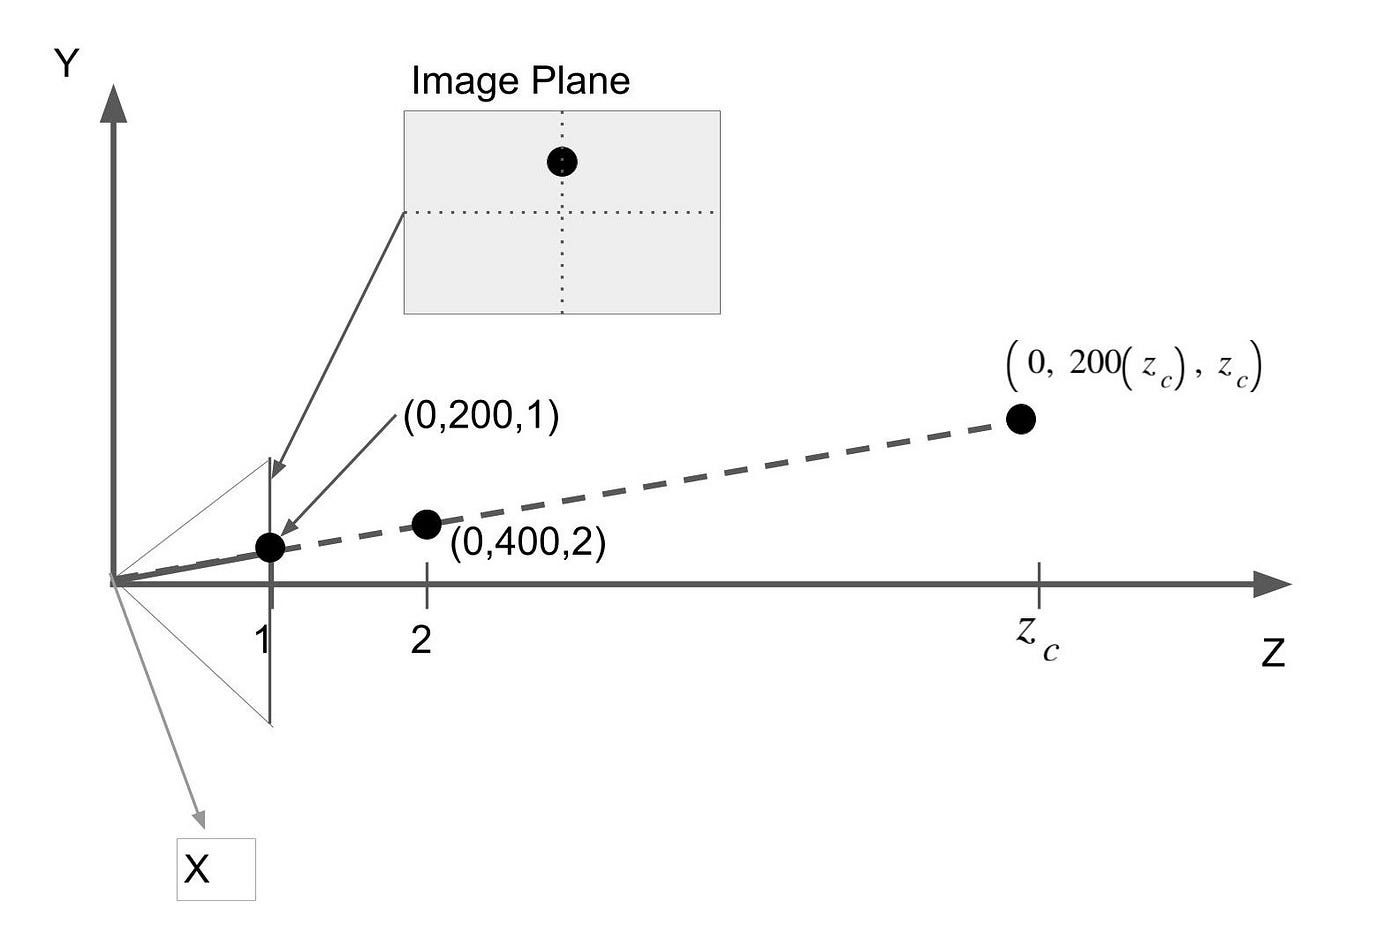
\includegraphics[width=\textwidth]{assets/ch3/camera projection illustration image.jpg}
	\caption{https://eugene-chian.medium.com/a-single-camera-3d-functions-fdec7ffa9a83}
	\label{camera projection illustration image}
\end{figure}
The following equation describes the relation between the real world points and the image points:
\begin{equation}
x = PX\label{x = PX}
\end{equation}
\subparagraph{Where:}
\begin{itemize}
	\item \textbf{x = [u, v, 1]$^T$} is the homogeneous coordinate of the 2D point in the image plane.
	\item \textbf{X = [x$_w$, y$_w$, z$_w$, 1]$^T$} is the homogeneous coordinate of the 3D point in the world coordinate system.
	\item \textbf{P = K$[R|t]$} is the camera projection matrix.
	\subparagraph{With:}
	\begin{itemize}
		\item \textbf{$[R|t]$} is the camera's extrinsic matrix, which "is a transformation matrix from the world coordinate system to the camera coordinate system" - Aqeel Anwar \cite{Aqeel Anwar}.
		
		R is a 3x3 matrix that represents the rotation of the object’s with respect to the camera. t is 3x1 vector describes the object's position relative to the camera.
		\begin{center} 
			\[
			[R|t] = \begin{bmatrix}
				R_{3\times3} & t_{3\times1}
			\end{bmatrix}_{(3\times4)}
			=
			\begin{bmatrix}
				r_{11} & r_{12} & r_{13} & t_{x}\\
				r_{21} & r_{22} & r_{23} & t_{y}\\
				r_{31} & r_{32} & r_{33} & t_{z}
			\end{bmatrix}
			\]
		\end{center}
		
		\item \textbf{K} is the camera's intrinsic matrix, which "is a transformation matrix that converts points from the camera coordinate system to the pixel coordinate system" - Aqeel Anwar \cite{Aqeel Anwar}. It contains camera's focal length(f$_x$, f$_y$) and the principal point(c$_x$, c$_y$) as follows:
		
		\begin{center} 
			$K = \begin{bmatrix}
				f_x & 0 & c_x\\
				0 & f_y & c_y\\
				0 & 0 & 1
			\end{bmatrix}$
		\end{center}
		
		Notice how the camera's intrinsic matrix cares only about the camera's internal parameters, while the extrinsic matrix does not.
	\end{itemize}
\end{itemize}

Now we can rewrite equation \ref{x = PX} as follows:

\begin{equation}
	s
	\begin{bmatrix}
		u\\v\\1
	\end{bmatrix}
	=
	\begin{bmatrix}
		f_x & 0 & c_x\\
		0 & f_y & c_y\\
		0 & 0 & 1
	\end{bmatrix}
	\begin{bmatrix}
		r_{11} & r_{12} & r_{13} & t_{x}\\
		r_{21} & r_{22} & r_{23} & t_{y}\\
		r_{31} & r_{32} & r_{33} & t_{z}
	\end{bmatrix}
	\begin{bmatrix}
		x_w\\y_w\\z_w\\1
	\end{bmatrix}
	\label{expanded form of x = PX}
\end{equation}
where s is a scale factor due to the homogeneous coordinates.

\begin{figure}[h] % [h] forces the figure to be placed exactly here in the text
	\centering
	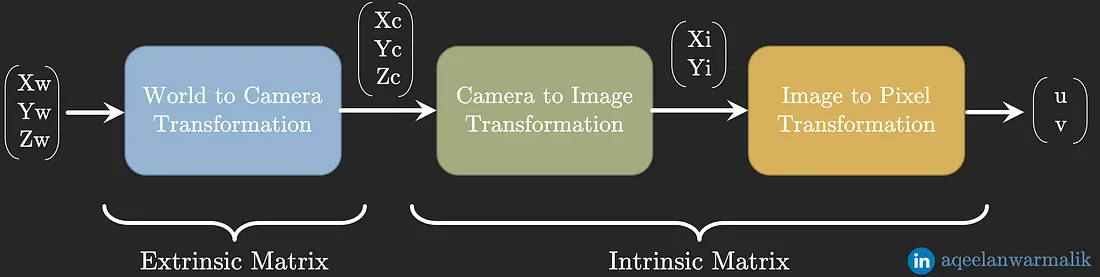
\includegraphics[width=\textwidth]{assets/ch3/Aqeel Anwar's camera's projection pipeline.png}
	\caption{Simple illustration for the camera's projection matrix made by Aqeel Anwar \cite{Aqeel Anwar}.1}
\end{figure}

After we understood the basics of how cameras project 3D world points into 2D images, we can use this knowledge to calculate the pose of an object, such as a QR code. At least four 3D points at the object need to be known, such as the four corners of a QR code in the world coordinate system. Then, the corresponding 2D projections in the image plane of these points need to be known. See figure \ref{QR code's known points} for illustration.

\begin{figure}[h] % [h] forces the figure to be placed exactly here in the text
	\centering
	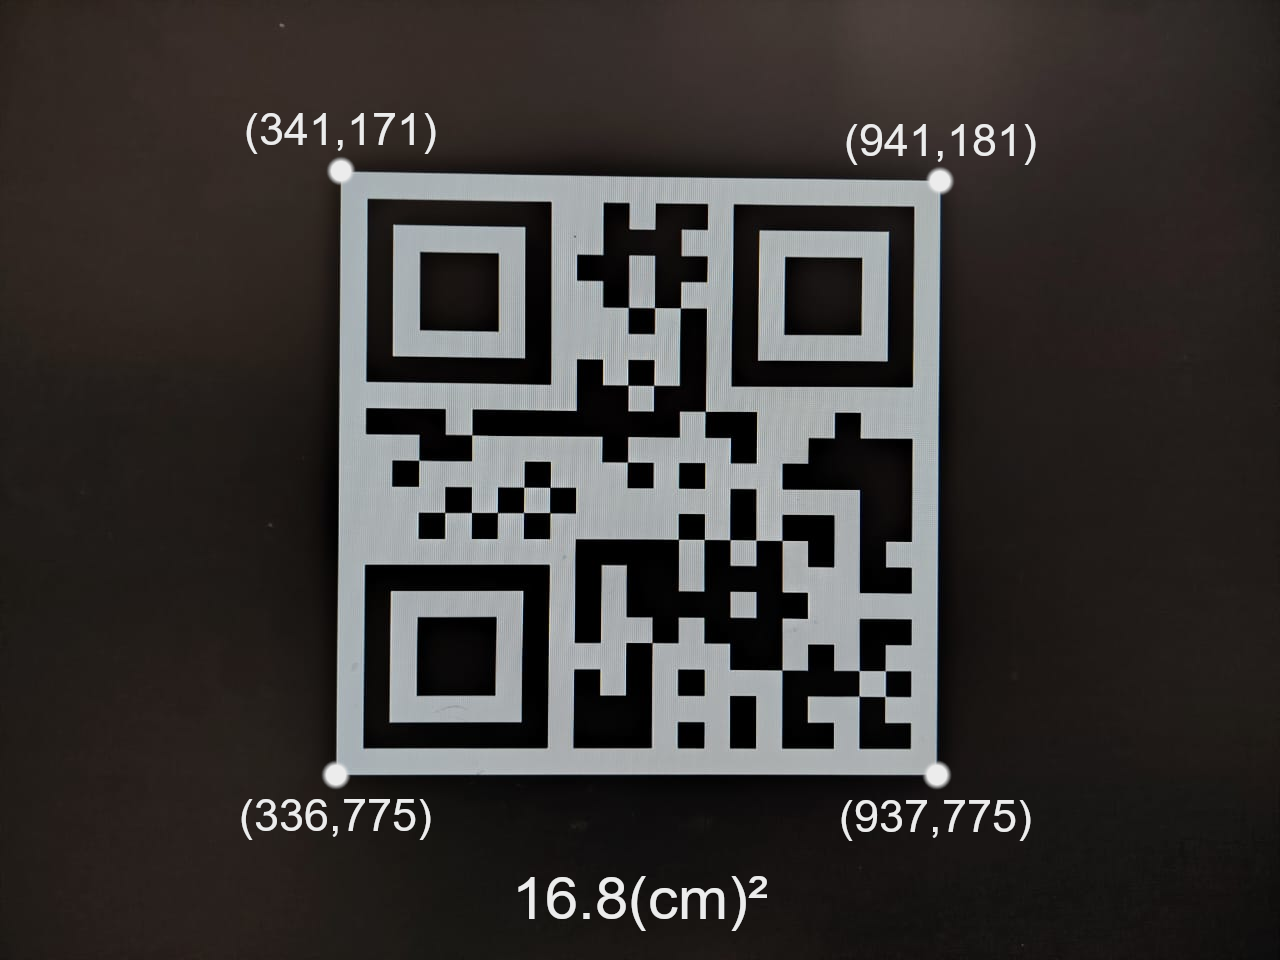
\includegraphics[width=330pt]{assets/ch3/QR code's known points/QR code's known points.png}
	\caption{This is a picture of a QR code that has the width/height of 16.8cm and its four corners points in the image coordinate system in pixels are known as it appears.}
	\label{QR code's known points}
\end{figure}

For more illustration, let us take the QR code at figure \ref{QR code's known points} as an example. The QR code's width/height is equal to 16.8cm in the real world coordinate system. Using this value, we will be able to extract the four corners 3D points in the real world coordinate system as follows:
\begin{equation}
	\begin{matrix}
		top-left-point = (-16.8/2, 16.8/2, 0) = (-8.4, 8.4, 0)\\
		top-right-point = (8.4, 8.4, 0)\\
		bottom-right-point = (-8.4, 8.4, 0)\\
		bottom-left-point = (-8.4, -8.4, 0)
	\end{matrix}
	\label{QR corner points relative to its center}
\end{equation}
For the sake of simplicity, the values at \ref{QR corner points relative to its center} are for a QR code with a global position value of (0,0,0).

After choosing some pairs of 3D points with their corresponding 2D projections, use equation \ref{expanded form of x = PX} for each pair as follows:

\begin{equation}
	s
	\begin{bmatrix}
		u_i\\v_i\\1
	\end{bmatrix}
	=
	\begin{bmatrix}
		f_x & 0 & c_x\\
		0 & f_y & c_y\\
		0 & 0 & 1
	\end{bmatrix}
	\begin{bmatrix}
		r_{11} & r_{12} & r_{13} & t_{x}\\
		r_{21} & r_{22} & r_{23} & t_{y}\\
		r_{31} & r_{32} & r_{33} & t_{z}
	\end{bmatrix}
	\begin{bmatrix}
		x_{w,i}\\y_{w,i}\\z_{w,i}\\1
	\end{bmatrix}
\nonumber\end{equation}
This yields two equations per point:
\begin{equation}
	u_i = \frac{f_x(r_{11}x_{w,i} + r_{12}y_{w,i} + r_{13}z_{w,i} + t_{x})}{r_{31}x_{w,i} + r_{32}y_{w,i} + r_{33}z_{w,i} + t_{z}} + c_x
\nonumber\end{equation}
\begin{equation}
	v_i = \frac{f_y(r_{21}x_{w,i} + r_{22}y_{w,i} + r_{23}z_{w,i} + t_{y})}{r_{31}x_{w,i} + r_{32}y_{w,i} + r_{33}z_{w,i} + t_{z}} + c_y
\nonumber\end{equation}

Finally, use the later equations to solve for R and t by using one of the PnP(Perspective-n-Point) algorithms. At the end, we will have the values of R and t which is the camera's extrinsic matrix that describes an object's rotation and translation relative to the camera. So, this is how to get the relative pose.

\subparagraph{PnP}
PnP is a classic approach in computer vision for determining the pose of a calibrated camera with respect to a set of known 3D points in the real world coordinate system and their corresponding 2D projection points. So in a nutshell a PnP algorithm takes three inputs: 3D points, 2D projection points, and intrinsic matrix to solve the camera's pose. There are several different PnP algorithms such as Direct Linear Transformation(DLT), Efficient PnP(EPnP), and RANSAC-PnP. 

\subparagraph{Camera Calibration}
\label{Camera Calibration Background}
Camera Calibration is the process of calculating the camera's focal length, principal point, and distortion coefficients. The basic idea behind camera calibration is to take multiple photos by the camera to a known pattern, then try to accurately locate some points at these photos. Then compare these estimated points to their physical locations of points in the calibration pattern (usually on a flat surface) in the real-world coordinate system. By comparing the 2D points in the images to their known 3D locations in the real-world coordinate system, we will be able to calculate accurate values of the camera's focal length, principal point, and distortion coefficients.

\begin{figure}[h] % [h] forces the figure to be placed exactly here in the text
	\centering
	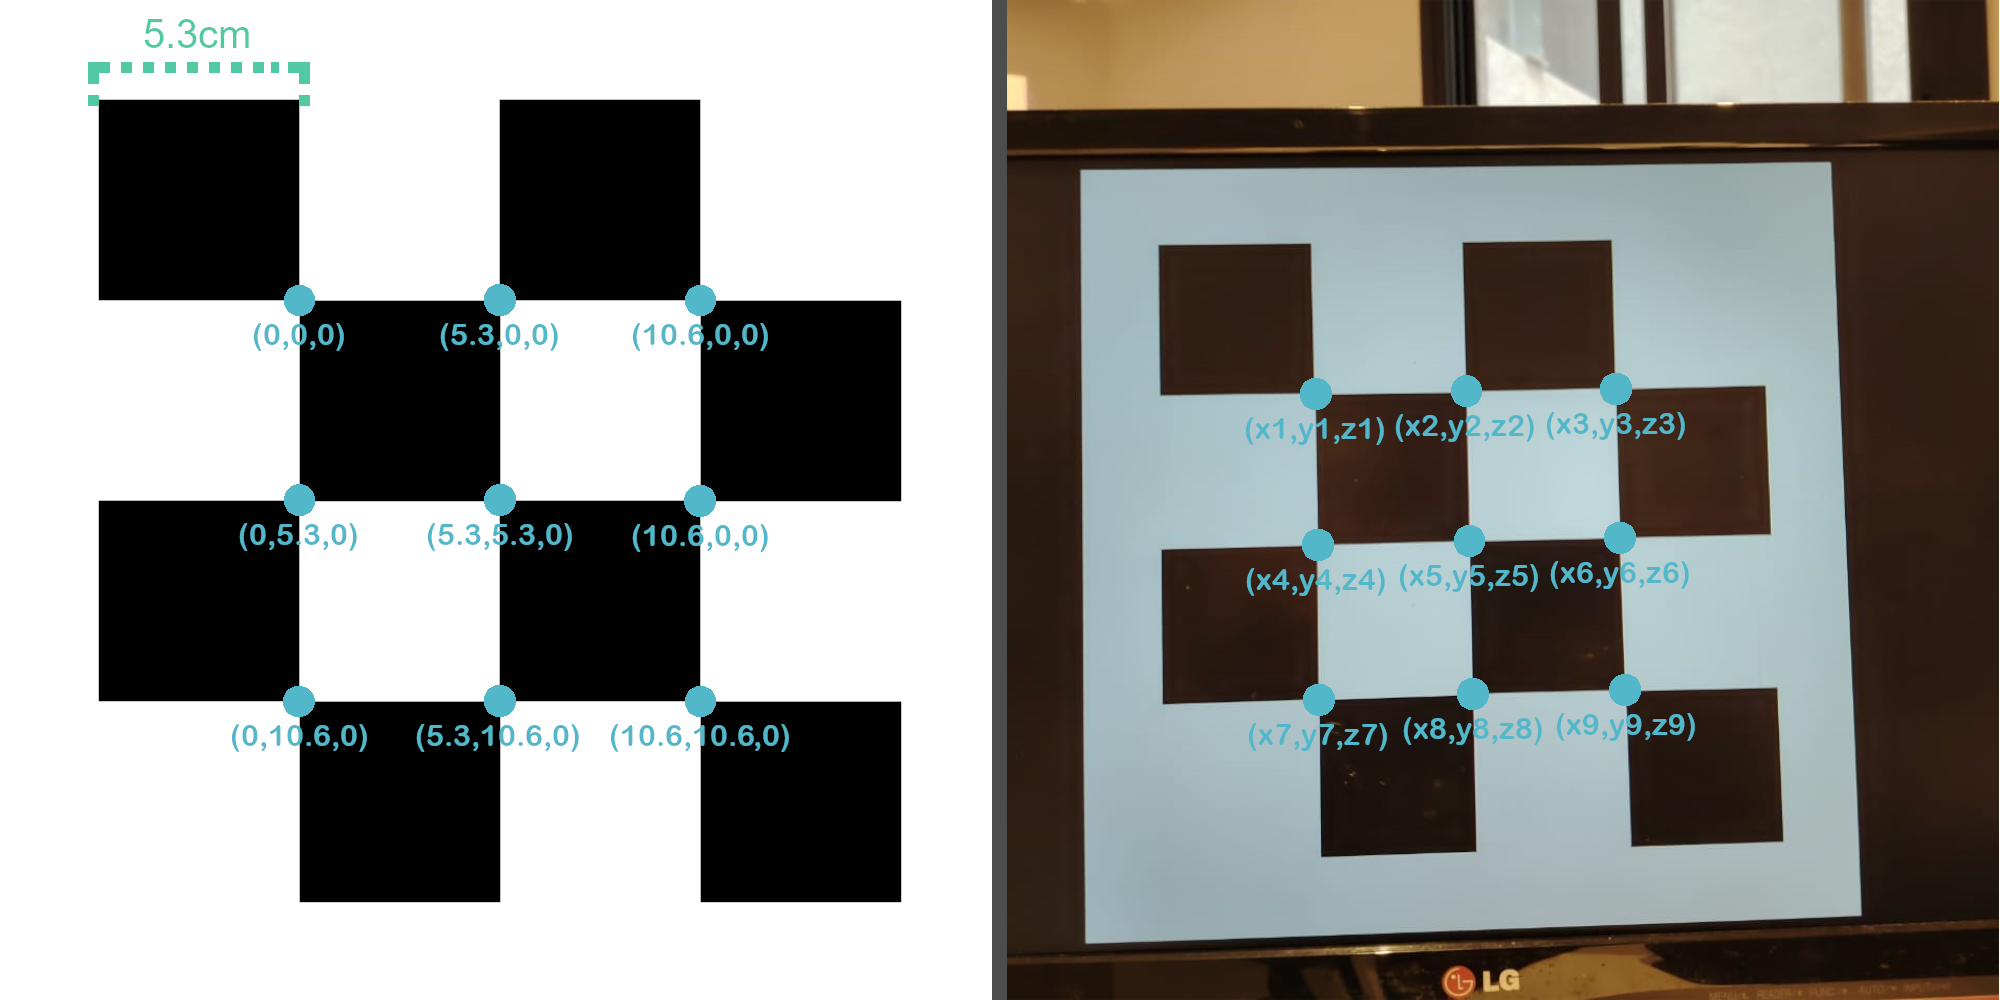
\includegraphics[width=\textwidth]{assets/ch3/calibration illustration image/calibration illustration image.png}
	\caption{ The left image represents the calibration pattern's real world inner points locations. While on the other hand, the right image shows the estimated inner  points locations. }
	\label{Calibration_Illustrator}
\end{figure}

\subparagraph{Libraries:}
\label{localization libraries BG}
\begin{itemize}
\item \textbf{Camera Libraries}:
There are several libraries for cameras in Android devices, such as Camera2, and CameraX. It is recommended for most developers to use CameraX library, since it supports the vast majority of Android devices, and provides a simple and easy to use API - unlike Camera2 - that spares users from dealing with compatibility issues and other low level details. See \cite{whichCameraLibToUse} for more info.
\end{itemize}
\begin{itemize}
	\item \textbf{Computer Vision Libraries}:
	\color{green}temporarily empty...\color{black}
\end{itemize}

While the pose estimation approach offers significantly higher accuracy, it requires greater computational resources due to additional processes, such as camera calibration to determine intrinsic parameters. This increased complexity makes the method more resource-intensive compared to the divided environment approach. However, it is suitable for applications where continuous and precise localization is essential.



